\subsubsection{Overall}
The Raspberry Pi Model 4B collects data from three devices--imaging sensor, GPS, and a current clamp. 
The imaging sensor counts the number of people inside the PRT car, the GPS hat tracks the current location of the PRT car, and the current clamp monitors the voltage and current being drawn by the PRT car. 
These three devices transfer their data to the Raspberry Pi. 
Once the Pi is stopped for about 5 seconds and has a Wi-Fi connection to WVU Encrypted, the data transfers to a SQL database hosted on a Google Cloud server instance. 
Next, a web application retrieves the data from the SQL database to visualize it, providing graphs and charts to analyze relationships between the data. 
The overall architecture is in Figure 2 and Figure 3, which represents the system functionality from top to bottom.

\begin{center}
    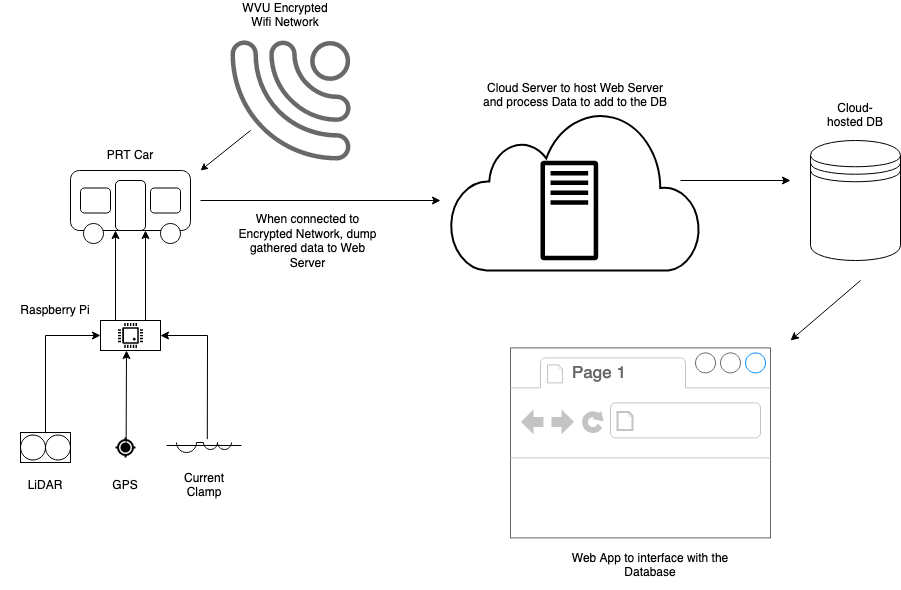
\includegraphics[width=0.5\textwidth]{Overall_Architecture.png}\\
    Fig 2. Overall Architecture
\end{center}

\begin{center}
    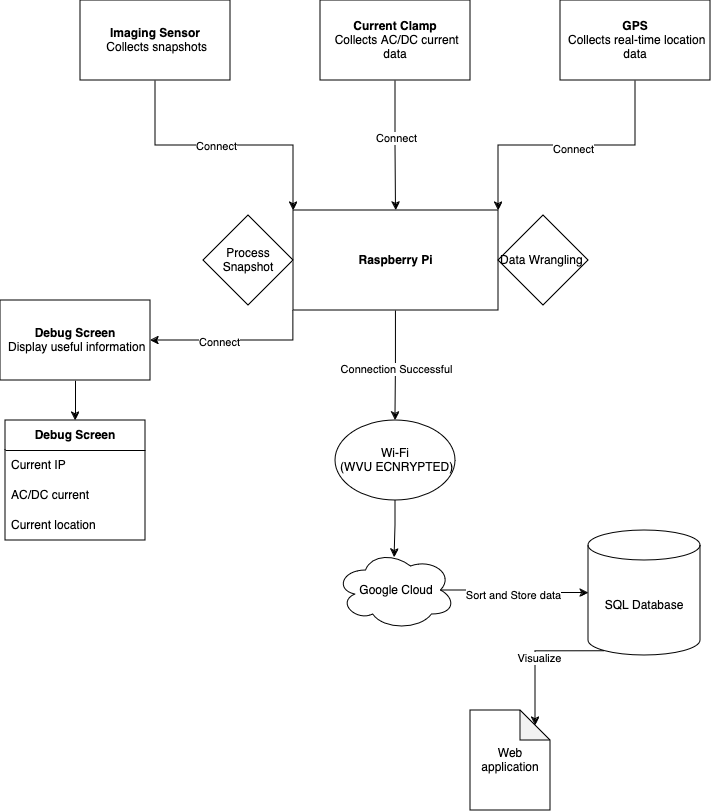
\includegraphics[width=0.5\textwidth]{System_Functionality.png}\\
    Fig 3. System Functionality
\end{center}

\subsubsection{Hardware}
Four devices fit onto the Raspberry Pi for the collection of data. 
The connections are shown below in Figure 4. 
The Pi communicates with the GPS for real-time location. 
The antenna plugs into the GPS and realizes the data collection. 
The current clamp collects AC voltage and current readings, recording it to the Pi.
A debug screen displays the GPS status, IP address, and the current AC reading for debugging purposes. 
The debug screen configures the subsystem, ensuring that the components work. 
Lastly, the imaging sensor collects snapshots of people for detecting the number of people in a PRT car. 
The snapshots go to the Raspberry Pi, where the Pi will use an algorithm to count the number of people in that snapshot.

\begin{center}
    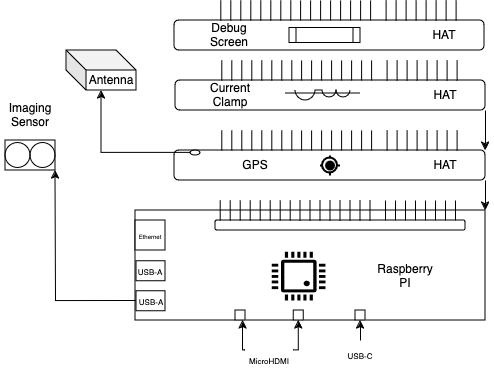
\includegraphics[width=0.5\textwidth]{Hardware_Architecture.png}\\
    Fig 4. Hardware Architecture
\end{center}

\subsubsection{Software}
When the Raspberry Pi obtains a Wi-Fi connection through WVU Encrypted and is at a standstill for 5 seconds or more, data goes to Google Cloud. 
Figure 5 represents the process of data transfer once Wi-Fi connects. 
The Google Cloud hosts a SQL database that sorts and stores all the metadata from the Pi system. 
A web application uses this sorted data from the SQL database, providing visualization through charts and graphs to highlight relationships in the data. 
The web application provides opportunities for identifying potential risks in the system, such as irregular AC current or voltage on a specific PRT car.

\begin{center}
    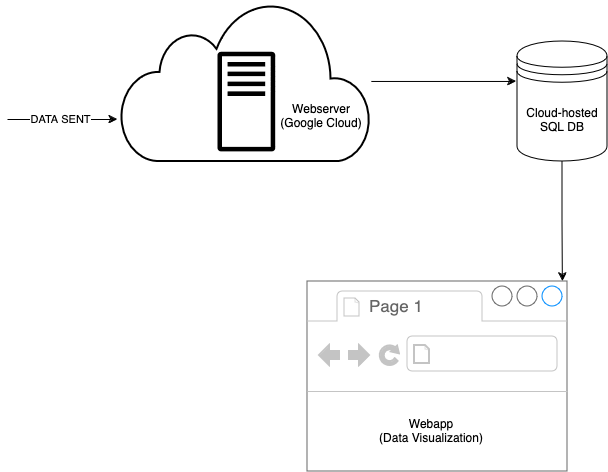
\includegraphics[width=0.5\textwidth]{Software_Architecture.png}\\
    Fig 5. Software Architecture
\end{center}